\documentclass[border=3pt]{standalone}
% Preâmbulo compartilhado pelos diagramas TikZ da aula
\usepackage[T1]{fontenc}
\usepackage[utf8]{inputenc}
\usepackage{lmodern}
\usepackage{amsmath}
\usepackage{xcolor}
\usepackage{tikz}
\usetikzlibrary{arrows.meta,angles,quotes,decorations.pathmorphing,calc,
                positioning,shapes.geometric,backgrounds,fit}

% Paleta (mesma dos SVGs originais)
\definecolor{dblue}{HTML}{2A5B8C}
\definecolor{dorange}{HTML}{B3541E}
\definecolor{dgreen}{HTML}{4A7C59}
\definecolor{dred}{HTML}{9C4B4B}
\definecolor{dcream}{HTML}{F4F1EA}
\definecolor{dshade}{HTML}{DDD7C9}

% Estilos comuns (prefixo d... para não colidir com chaves internas do pgf)
\tikzset{
  >={Stealth[length=2mm]},
  dguide/.style={gray!55, dashed, line width=0.4pt},
  daxis/.style={gray!60, line width=0.7pt, ->},
  dbody/.style={fill=black!3, draw=black!80, line width=1pt},
  dacc/.style={draw=dblue, line width=1pt},
  dlbl/.style={black!55, font=\small},
  dsub/.style={black!45, font=\footnotesize},
  dstate/.style={circle, draw=black!80, fill=dcream, line width=1pt,
                 minimum size=17mm, font=\large, inner sep=1pt},
  dobs/.style={circle, draw=black!80, fill=dshade, line width=1pt,
               minimum size=14mm, font=\large, inner sep=1pt},
  dbox/.style={rounded corners=2pt, draw=black!80, fill=dcream, line width=1pt,
               align=center, inner sep=6pt},
  dtrans/.style={->, dblue, line width=1pt},
  dmeas/.style={->, dorange, line width=1pt},
}

\begin{document}
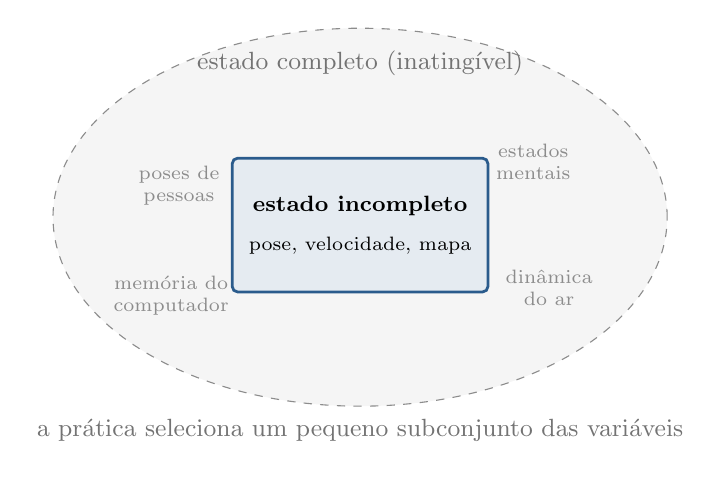
\begin{tikzpicture}[x=1cm,y=1cm]

  % estado completo: nuvem grande
  \node[draw=black!45, dashed, ellipse, minimum width=7.8cm, minimum height=4.8cm,
        fill=black!4] (full) at (0,0) {};
  \node[black!55, font=\small] at (0,1.95) {estado completo (inatingível)};

  % itens dentro
  \foreach \p/\t in {{-2.3,0.4}/{poses de\\pessoas}, {2.2,0.7}/{estados\\mentais},
                     {-2.4,-1.0}/{memória do\\computador}, {2.4,-0.9}/{dinâmica\\do ar}}
    \node[black!45, font=\scriptsize, align=center] at (\p) {\t};

  % subconjunto selecionado
  \node[dbox, fill=dblue!12, draw=dblue, minimum width=3.1cm, minimum height=1.7cm]
       (sub) at (0,-0.1) {\footnotesize\textbf{estado incompleto}\\[2pt]\scriptsize pose, velocidade, mapa};

  \node[dlbl] at (0,-2.7) {a prática seleciona um pequeno subconjunto das variáveis};

\end{tikzpicture}
\end{document}
